\documentclass[11pt,a4paper]{article}

% Packages for formatting and layout
\usepackage{geometry}  % Adjust margins
\geometry{margin=0.7in}
\usepackage{setspace}  % For line spacing
\usepackage{graphicx, wrapfig}
\graphicspath{ {./assets/} }
\usepackage{amsmath}   % For mathematical expressions
\usepackage{hyperref}  % For hyperlinks
\usepackage{enumitem}  % For custom lists

% Title information
\title{Predicting news truthfulness through graph-based retweet patterns.}
\author{Baggio Davide 2122547 \\ Martinez Zoren 2123873 \\ Brocheton Damien 2133034}
\date{}

\usepackage{etoolbox}
\makeatletter
\patchcmd{\@maketitle}{\null\vskip 2em}{}{}{}
\makeatother

\begin{document}

% Title Page
\maketitle

\section*{Project Idea}

The main objective and idea of the project haven't changed since the proposal. The purpose of this project is to prove whether it’s possible to classify news as real or fake based solely on the ”pure” retweet
graph structure, independently of user metadata.

\section*{Implementation}

During this period of time the group has implemented some basic programs in Python (using NetworkX\cite{networkx}) in order to extract useful information about the Graphs of news retweets, such as:

\begin{itemize}
	\setlength\itemsep{-0.3em}
	\item \textbf{Diameter}
	\item \textbf{Max Degree}
	\item \textbf{Standard Deviation of Timestamps}
	\item \textbf{Degree Centrality}
	\item \textbf{Closeness Centrality}
	\item \textbf{PageRank}
\end{itemize}

A system of prediction based on score has also being implemented. It gets some graphs data as input and determines how much it deviates from the averages calculated with previous algorithms.

%\begin{wrapfigure}{r}{0.5\textwidth}
	\begin{center}
	  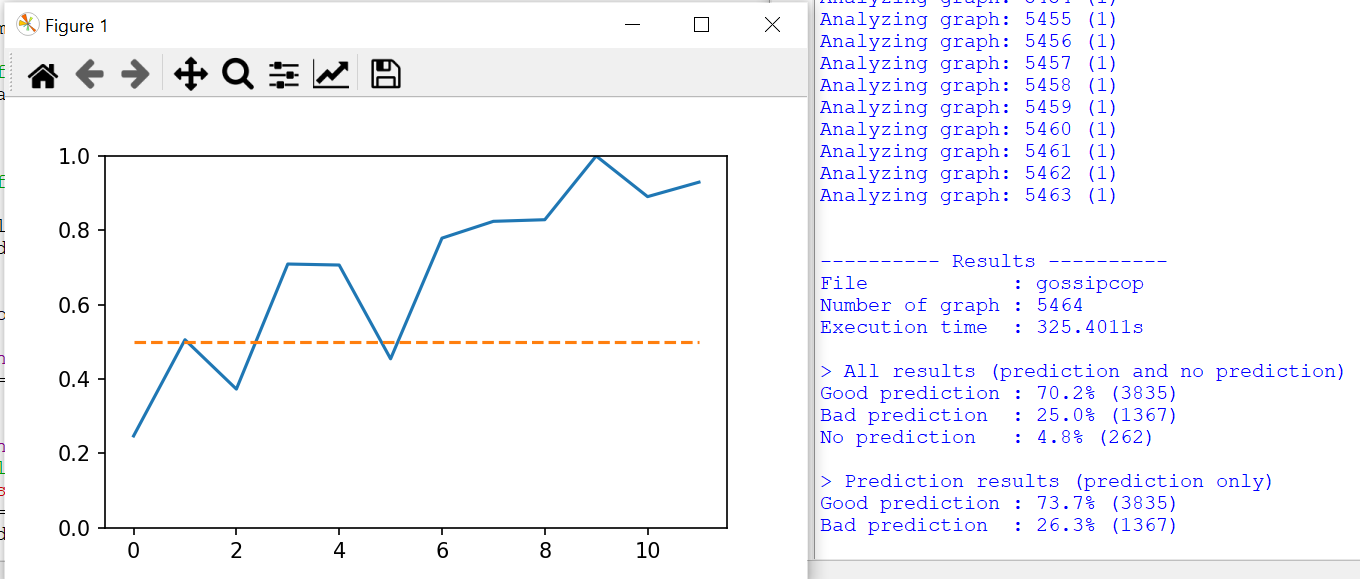
\includegraphics[width=0.8\textwidth]{results_gos}
	\end{center}
%\end{wrapfigure}

The image above is just an example on how it can display the prediction. We should obviously split the data into training and test sets, but for now, from what we can see, there is a correlation between the data extracted from the graphs and their actual label (Real / Fake).

Implementation published in the github repository\cite{github}

\section*{Machine Learning}

As we discovered the correlation between the data and the graphs label, the last part we need to implement is the machine learning model that can actually infer the label of a graph given as input. We have been discussing about the models we should use and the ideas haven't changed.
We are talking about using:
\begin{itemize}
	\setlength\itemsep{-0.3em}
	\item \textbf{Support Vector Machine}
	\item \textbf{Feed Forward Neural Network}
	\item \textbf{Random Forest}
\end{itemize}

As the project move towards the final results we might try different models in order to find the best predictors.

\newpage

\begin{thebibliography}{9}
	%\bibitem{rec_studies} Yi Han, Shanika Karunasekeran, Christopher Leckie\\"Graph Neural Networks with Continual Learning for Fake News Detection from Social Media",\\ \url{https://arxiv.org/pdf/2007.03316}, 2020.
	%\bibitem{dataset} Dataset: \url{https://github.com/safe-graph/GNN-FakeNews/tree/main},\\\url{https://drive.google.com/drive/folders/1OslTX91kLEYIi2WBnwuFtXsVz5SS_XeR?usp=sharing}
	%\bibitem{data_paper} Kai Shu, Deepak Mahudeswaran, Suhang Wang, Dongwon Lee and Huan Liu\\"FakeNewsNet: A Data Repository with News Content, Social Context and Spatiotemporal Information for Studying Fake News on Social Media",\\ \url{https://arxiv.org/pdf/1809.01286}, 2019
	\bibitem{networkx} NetworkX library: \url{https://networkx.org/documentation/stable/}

	\bibitem{github} Github Repository: \url{https://github.com/davidebaggio/LFN_proj}
\end{thebibliography}

\newpage

\section*{Contribution}
Contributors:
\begin{itemize}
	\setlength\itemsep{-0.3em}
	\item Baggio Davide ($\frac{1}{3}$ of the work): All the work documented in the proposal, finishing the implementation of the extraction of information about the dataset, preparing the data into a ".csv" ready for the ML models.
	\item Martinez Zoren ($\frac{1}{3}$ of the work): All the work documented in the proposal, starting to implement the firts ML models
	\item Brocheton Damien ($\frac{1}{3}$ of the work): All the work documented in the proposal, finishing the implementation of the probabilistic algorithm that gives a score to a graph in order to predict if it is a Real or Fake news.
\end{itemize}

\end{document}
